\documentclass[../zhang_thesis.tex]{subfiles}
\begin{document}

\chapter{Filtering Results}

%%%%%%%%%%%%%%%%%%%%%%%%%%%%%%%%%%%%%%%%%%%%%%%%%%%%%%%%%%%%%%%

\section{Performance Measures}

This study was concerned with the accuracy and speed of the nonlinear filters for estimation of the SOC. The accuracy of the estimation was measured using the mean RMSE (MRMSE). Recall that the state variable $x_1$ represents the SOC. The other two state variables don't directly represent physical properties of the battery and are less useful in battery management, so they are ignored in determining the RMSE. However, the filters probably resulted in comparable error in their
estimates as in the SOC estimates. For the SOC, the RMSE is defined as
\begin{equation}
    \mathrm{RMSE}(kT_s) = \sqrt{ \frac{1}{N_\text{trials}} \sum_{j=1}^{N_\text{trials}} \Big( \hat{x}_1^{(j)}(kT_s) - x_1^{(j)}(kT_s) \Big)^2 },
\end{equation}
where $T_s$ is the sample period, the superscript $(j)$ indicates the $j$th Monte Carlo trial, and the squared error is averaged over the Monte Carlo trials. Additionally, recall that $N_\text{trials}=100$ Monte Carlo trials were used in this study. Note that the defined RMSE is a function of discrete time steps. Then, the MRMSE is the mean of the RMSE over the time steps, giving
\begin{equation}
    \mathrm{MRMSE} = \frac{1}{N} \sum_{k=1}^N \mathrm{RMSE}(kT_s),
\end{equation}
where $N$ is the total number of time steps at which the filtering was performed. Note that the MRMSE is a nonnegative number, and it is desirable for a filter to produce an estimate with a small MRMSE, indicating a more accurate estimate. An additional measure of accuracy is the number of trials in which the filter estimate diverged. A divergence was considered to be an absolute error in the estimated SOC greater than $0.1~\mathrm{V}$ or any failure in the filtering process, such
as due to a non-invertible matrix or a non-positive definite covariance matrix. In addition, after a filter failed in a trial, the filtering process was halted for that trial, and the remainder of the SOC values were assumed to be the worst case of zero, i.e.\ a fully discharged battery. Furthermore, the speed of a filter was measured using the CPU time it took to complete the Monte Carlo trials. This time is the sum of the times used by the filter program on each of the CPU cores. The use of
the CPU time results in less variability between runs compared to the clock time. In addition, the time taken to read and write the data was not counted, since that time should be the same for all the filters and this study was concerned about the computational complexity of the filters.

The remainder of this chapter shows the filtering results for sampling periods $T_s$ of 30, 150, and 300 seconds. Additionally, integration steps of $M=1,2,4,\dots,256$ were used for each sampling period. For each sampling period, the number of divergences and filtering times are displayed as a function of the number of integration steps. Then, the MRMSEs are plotted for those integration steps that have zero divergences. Finally, the RMSEs are plotted as a function of time for the
least and most numbers of integration steps that produce zero divergences.

\section{Sampling Period of 30 Seconds}

From \cref{tab:div_30}, it can be seen that the filters had no divergences for $M=4,\dots,64$. For small $M$, all filters diverged, as expected. However, the UKF and the CKF3 also diverged for large $M$, which can be explained by numerical problems arising from the large number of integration steps. The times shown in \cref{tab:time_30} show that the EKF was by far the fastest, about three to four times the speed of the next fastest, the SLF. Additionally, the EKF was about five times the
speed of the UKF and the CKF3 and more than twelve times the speed of the CKF5. The slowness of the CKF5 was a result of using about three times as many cubature points as the CKF3.

\begin{table}[h]
\centering
\caption{Number of divergences in 100 Monte Carlo runs for $T_s=30$~s as a function of number of integration steps $M$}
\begin{tabular}{@{}l*{9}{c}@{}}
\toprule
Filter/$M$ & 1   & 2   & 4 & 8 & 16 & 32 & 64 & 128 & 256 \\
\midrule
EKF        & 88  & 56  & 0 & 0 & 0  & 0 & 0 & 0 & 0   \\
UKF        & 91  & 8   & 0 & 0 & 0  & 0 & 0 & 3 & 26  \\
CKF3       & 96  & 6   & 0 & 0 & 0  & 0 & 0 & 0 & 1   \\
CKF5       & 100 & 95  & 0 & 0 & 0  & 0 & 0 & 0 & 0   \\
SLF        & 100 & 100 & 0 & 0 & 0  & 0 & 0 & 0 & 0   \\
\bottomrule
\end{tabular}
\label{tab:div_30}
\end{table}

\begin{table}[h]
\centering
\caption{Filtering time in seconds for 100 Monte Carlo runs for $T_s=30$~s as a function of number of integration steps $M$}
\begin{tabular}{@{}lccccccccc@{}}
\toprule
Filter/$M$ & 1     & 2     & 4     & 8     & 16    & 32    & 64    & 128   & 256   \\ \midrule
EKF        & 4.253 & 5.017 & 4.951 & 9.708 & 19.32 & 38.8  & 77.11 & 154   & 307.9 \\
UKF        & 4.834 & 11.85 & 23.65 & 47.24 & 93.46 & 186.5 & 373.1 & 732.9 & 1274  \\
CKF3       & 4.221 & 10.61 & 21.1  & 41.33 & 82.57 & 165   & 328.2 & 657.9 & 1317  \\
CKF5       & 9.533 & 28.82 & 59.49 & 117.8 & 234.9 & 468.8 & 937.9 & 1873  & 3748  \\
SLF        & 4.521 & 6.52  & 16.35 & 32.11 & 63.43 & 126.7 & 252.1 & 503.5 & 1006  \\ \bottomrule
\end{tabular}
\label{tab:time_30}
\end{table}

\cref{fig:mrmse_30} shows the MRMSE as a function of the number of integration steps over the divergence-free range. It can be see that the EKF result showed a decrease over this range as expected. However, the other results had minimum error at $M=16$, with an increase in error for larger $M$. This could be due to numerical errors that also caused divergences for large $M$ in the case of the UKF and the CKF3. The global minimum error was produced by both the CKF5 and the SLF at $M=16$.
Interestingly, the EKF resulted in the largest error for that number of integration steps out of all the filters.

\begin{figure}[ht]
\centering
%% generated by laprint.m
%
%
% text strings:
\psfrag{s05}[t][t]{\color[rgb]{0,0,0}\setlength{\tabcolsep}{0pt}\begin{tabular}{c}$\log_2 (M)$\end{tabular}}%
\psfrag{s06}[b][b]{\color[rgb]{0,0,0}\setlength{\tabcolsep}{0pt}\begin{tabular}{c}MRMSE\end{tabular}}%
\psfrag{s10}[][]{\color[rgb]{0,0,0}\setlength{\tabcolsep}{0pt}\begin{tabular}{c} \end{tabular}}%
\psfrag{s11}[][]{\color[rgb]{0,0,0}\setlength{\tabcolsep}{0pt}\begin{tabular}{c} \end{tabular}}%
\psfrag{s12}[l][l]{\color[rgb]{0,0,0}SLF}%
\psfrag{s13}[l][l]{\color[rgb]{0,0,0}EKF}%
\psfrag{s14}[l][l]{\color[rgb]{0,0,0}UKF}%
\psfrag{s15}[l][l]{\color[rgb]{0,0,0}CKF3}%
\psfrag{s16}[l][l]{\color[rgb]{0,0,0}CKF5}%
\psfrag{s17}[l][l]{\color[rgb]{0,0,0}SLF}%
%
% xticklabels:
\psfrag{x01}[t][t]{2}%
\psfrag{x02}[t][t]{3}%
\psfrag{x03}[t][t]{4}%
\psfrag{x04}[t][t]{5}%
\psfrag{x05}[t][t]{6}%
%
% yticklabels:
\psfrag{v01}[r][r]{4.8}%
\psfrag{v02}[r][r]{5}%
\psfrag{v03}[r][r]{5.2}%
\psfrag{v04}[r][r]{5.4}%
\psfrag{v05}[r][r]{5.6}%
\psfrag{v06}[r][r]{5.8}%
\psfrag{v07}[r][r]{6}%
\psfrag{ypower2}[Bl][Bl]{$\times 10^{-3}$}%
%
% Figure:
%
% End mrmse_30.tex

\psfragfig[width=15cm]{chapter-3/figures/mrmse_30}
\caption{MRMSE of SOC estimation for $T_s=30$~s as a function of number of integration steps $M$.}
\label{fig:mrmse_30}
\end{figure}

For comparison purposes, the RMSEs at $M=4$ and $64$ are shown in \cref{fig:rmse_30_4,fig:rmse_30_64}. The period of high error corresponds to the high-rate charge and discharge period that resulted in the strongest nonlinear effect. For $M=4$, the EKF had lower error initially during the high-rate charge and discharge period from about $k=1900$ to $2300$, but its error reached those of the other filters near the end of that period. The other filters had very comparable errors. For $M=64$, the EKF
had higher median error, but its lower worst case error resulted in the slightly lower MRMSE. The other filters were again very close in error, with the UKF having slightly higher error on average.

\begin{figure}[h]
\centering
%\input{chapter-3/figures/rmse_30_4}
\pstool[width=15cm]{chapter-3/figures/rmse_30_4}{\input{chapter-3/figures/rmse_30_4.tex}}
\caption{RMSE of SOC estimation for $T_s=30$~s and $M=4$.}
\label{fig:rmse_30_4}
\end{figure}

\begin{figure}
\centering
%\input{chapter-3/figures/rmse_30_64}
\pstool[width=15cm]{chapter-3/figures/rmse_30_64}{\input{chapter-3/figures/rmse_30_64.tex}}
\caption{RMSE of SOC estimation for $T_s=30$~s and $M=64$.}
\label{fig:rmse_30_64}
\end{figure}

\clearpage

\section{Sampling Period of 150 Seconds}

From \cref{tab:div_150}, it can be seen that the filters had no divergences for $M=16,\dots,256$. For small $M$, all filters diverged, as expected. For large $M$, there were no divergences, unlike with $T_s=30$ seconds. The times in \cref{tab:time_150} show that the EKF was again the fastest with a similar ratio between the speeds as with $T_s=30$ seconds. 

\begin{table}[h]
\centering
\caption{Number of divergences in 100 Monte Carlo runs for $T_s=150$~s as a function of number of integration steps $M$}
\begin{tabular}{@{}l*{9}{c}@{}}
\toprule
Filter/$M$ & 1   & 2   & 4   & 8   & 16 & 32 & 64 & 128 & 256 \\
\midrule
EKF        & 100 & 100 & 98  & 77  & 0  & 0  & 0  & 0   & 0   \\
UKF        & 100 & 100 & 100 & 100 & 0  & 0  & 0  & 0   & 0   \\
CKF3       & 100 & 100 & 100 & 100 & 0  & 0  & 0  & 0   & 0   \\
CKF5       & 100 & 100 & 100 & 100 & 0  & 0  & 0  & 0   & 0   \\
SLF        & 100 & 100 & 100 & 100 & 0  & 0  & 0  & 0   & 0   \\
\bottomrule
\end{tabular}
\label{tab:div_150}
\end{table}

\begin{table}[h]
\centering
\caption{Filtering time in seconds for 100 Monte Carlo runs for $T_s=150$~s as a function of number of integration steps $M$}
\begin{tabular}{@{}lccccccccc@{}}
\toprule
Filter/$M$ & 1      & 2     & 4     & 8     & 16    & 32    & 64    & 128   & 256   \\ \midrule
EKF        & 0.544  & 2.359 & 6.297 & 7.787 & 3.868 & 7.753 & 15.49 & 30.97 & 61.67 \\
UKF        & 0.6749 & 1.185 & 2.414 & 6.983 & 18.81 & 37.53 & 74.89 & 149.8 & 299.2 \\
CKF        & 0.499  & 1.173 & 2.147 & 6.098 & 16.49 & 33.09 & 66.08 & 131.9 & 264.1 \\
CKF5       & 2.949  & 5.709 & 10.93 & 22.49 & 47.34 & 94.14 & 188.2 & 377.6 & 753.7 \\
SLF        & 0.873  & 1.655 & 3.217 & 6.352 & 12.7  & 25.39 & 50.63 & 101   & 201.9 \\ \bottomrule
\end{tabular}
\label{tab:time_150}
\end{table}

\cref{fig:mrmse_150} shows the MRMSE as a function of the number of integration steps over the divergence-free range. It can be seen that the errors decreased as the number of integration steps increased, and the rate of decrease was roughly the same for all five filters. The EKF resulted in the least error by far, with its MRMSE at $M=16$ approximately equal to the MRMSEs of the other filters at $M=256$. For small $M$, the UKF had the second smallest error, and the two CKFs and the SLF
approximately tied for the most error. For large $M$, the CKF5 and the SLF had the second smallest error, being trailed by the CKF3 and then the UKF.

\begin{figure}[ht]
\centering
%\input{chapter-3/figures/mrmse_150}
\psfragfig[width=15cm]{chapter-3/figures/mrmse_150}
\caption{MRMSE of SOC estimation for $T_s=150$~s as a function of number of integration steps $M$.}
\label{fig:mrmse_150}
\end{figure}

For comparison purposes, the RMSEs at $M=16$ and $256$ are shown in \cref{fig:rmse_150_16,fig:rmse_150_256}. The period of high error corresponds to the high-rate charge and discharge period that resulted in the strongest nonlinear effect. For both sampling periods shown, the EKF had much lower error over the high-rate period and during the idle periods at the end of the simulation. For $M=16$, the UKF had higher error than the CKFs and the SLF, which were approximately equal in error, until about $k=350$ and then had lower error for
larger $k$. For $M=256$, the UKF had higher error than the CKFs and the SLF after about $k=380$ and about the same error before. The CKFs and the SLF were again approximately equal in error, with the CKF3 showing a small deviation from $k=290$ to $350$.

\begin{figure}[h]
\centering
%% generated by laprint.m
%
%
% text strings:
\psfrag{s05}[b][b]{\color[rgb]{0,0,0}\setlength{\tabcolsep}{0pt}\begin{tabular}{c}RMSE\end{tabular}}%
\psfrag{s06}[t][t]{\color[rgb]{0,0,0}\setlength{\tabcolsep}{0pt}\begin{tabular}{c}$k$\end{tabular}}%
\psfrag{s10}[][]{\color[rgb]{0,0,0}\setlength{\tabcolsep}{0pt}\begin{tabular}{c} \end{tabular}}%
\psfrag{s11}[][]{\color[rgb]{0,0,0}\setlength{\tabcolsep}{0pt}\begin{tabular}{c} \end{tabular}}%
\psfrag{s12}[l][l]{\color[rgb]{0,0,0}SLF}%
\psfrag{s13}[l][l]{\color[rgb]{0,0,0}EKF}%
\psfrag{s14}[l][l]{\color[rgb]{0,0,0}UKF}%
\psfrag{s15}[l][l]{\color[rgb]{0,0,0}CKF3}%
\psfrag{s16}[l][l]{\color[rgb]{0,0,0}CKF5}%
\psfrag{s17}[l][l]{\color[rgb]{0,0,0}SLF}%
%
% xticklabels:
\psfrag{x01}[t][t]{0}%
\psfrag{x02}[t][t]{100}%
\psfrag{x03}[t][t]{200}%
\psfrag{x04}[t][t]{300}%
\psfrag{x05}[t][t]{400}%
\psfrag{x06}[t][t]{500}%
\psfrag{x07}[t][t]{600}%
\psfrag{x08}[t][t]{700}%
%
% yticklabels:
\psfrag{v01}[r][r]{0}%
\psfrag{v02}[r][r]{0.005}%
\psfrag{v03}[r][r]{0.01}%
\psfrag{v04}[r][r]{0.015}%
\psfrag{v05}[r][r]{0.02}%
\psfrag{v06}[r][r]{0.025}%
\psfrag{v07}[r][r]{0.03}%
\psfrag{v08}[r][r]{0.035}%
%
% Figure:
%
% End rmse_150_16.tex

\pstool[width=15cm]{chapter-3/figures/rmse_150_16}{% generated by laprint.m
%
%
% text strings:
\psfrag{s05}[b][b]{\color[rgb]{0,0,0}\setlength{\tabcolsep}{0pt}\begin{tabular}{c}RMSE\end{tabular}}%
\psfrag{s06}[t][t]{\color[rgb]{0,0,0}\setlength{\tabcolsep}{0pt}\begin{tabular}{c}$k$\end{tabular}}%
\psfrag{s10}[][]{\color[rgb]{0,0,0}\setlength{\tabcolsep}{0pt}\begin{tabular}{c} \end{tabular}}%
\psfrag{s11}[][]{\color[rgb]{0,0,0}\setlength{\tabcolsep}{0pt}\begin{tabular}{c} \end{tabular}}%
\psfrag{s12}[l][l]{\color[rgb]{0,0,0}SLF}%
\psfrag{s13}[l][l]{\color[rgb]{0,0,0}EKF}%
\psfrag{s14}[l][l]{\color[rgb]{0,0,0}UKF}%
\psfrag{s15}[l][l]{\color[rgb]{0,0,0}CKF3}%
\psfrag{s16}[l][l]{\color[rgb]{0,0,0}CKF5}%
\psfrag{s17}[l][l]{\color[rgb]{0,0,0}SLF}%
%
% xticklabels:
\psfrag{x01}[t][t]{0}%
\psfrag{x02}[t][t]{100}%
\psfrag{x03}[t][t]{200}%
\psfrag{x04}[t][t]{300}%
\psfrag{x05}[t][t]{400}%
\psfrag{x06}[t][t]{500}%
\psfrag{x07}[t][t]{600}%
\psfrag{x08}[t][t]{700}%
%
% yticklabels:
\psfrag{v01}[r][r]{0}%
\psfrag{v02}[r][r]{0.005}%
\psfrag{v03}[r][r]{0.01}%
\psfrag{v04}[r][r]{0.015}%
\psfrag{v05}[r][r]{0.02}%
\psfrag{v06}[r][r]{0.025}%
\psfrag{v07}[r][r]{0.03}%
\psfrag{v08}[r][r]{0.035}%
%
% Figure:
%
% End rmse_150_16.tex
}
\caption{RMSE of SOC estimation for $T_s=150$~s and $M=16$.}
\label{fig:rmse_150_16}
\end{figure}

\begin{figure}
\centering
%\input{chapter-3/figures/rmse_150_256}
\pstool[width=15cm]{chapter-3/figures/rmse_150_256}{\input{chapter-3/figures/rmse_150_256.tex}}
\caption{RMSE of SOC estimation for $T_s=150$~s and $M=256$.}
\label{fig:rmse_150_256}
\end{figure}

\clearpage

\section{Sampling Period of 300 Seconds}

From \cref{tab:div_300}, it can be seen that the filters had no divergences for $M=64,\dots,256$. This is a smaller divergence-free range than before due to the long sampling period. The CKF5 and the SLF were the best in terms of divergences, followed by the EKF and the CKF3. The UKF had more numerical problems than the other filters, with some divergences still occurring for $M=32$. The times shown in \cref{tab:time_300} show that the EKF is again the fastest with a similar ratio between the speeds as with the other two sampling periods. 

\begin{table}[h]
\centering
\caption{Number of divergences in 100 Monte Carlo runs for $T_s=300$~s as a function of number of integration steps $M$}
\begin{tabular}{@{}l*{9}{c}@{}}
\toprule
Filter/$M$ & 1   & 2   & 4   & 8   & 16  & 32 & 64 & 128 & 256 \\
\midrule
EKF        & 100 & 100 & 100 & 100 & 71  & 0  & 0  & 0   & 0   \\
UKF        & 100 & 100 & 100 & 100 & 99  & 5  & 0  & 0   & 0   \\
CKF3       & 100 & 100 & 100 & 100 & 99  & 0  & 0  & 0   & 0   \\
CKF5       & 100 & 100 & 100 & 100 & 0   & 0  & 0  & 0   & 0   \\
SLF        & 100 & 100 & 100 & 100 & 0   & 0  & 0  & 0   & 0   \\
\bottomrule
\end{tabular}
\label{tab:div_300}
\end{table}

\begin{table}[h]
\centering
\caption{Filtering time in seconds for 100 Monte Carlo runs for $T_s=300$~s as a function of number of integration steps $M$}
\begin{tabular}{@{}lccccccccc@{}}
\toprule
Filter/$M$ & 1     & 2     & 4     & 8     & 16    & 32    & 64    & 128   & 256   \\ \midrule
EKF        & 0.39  & 0.763 & 2.998 & 7.169 & 8.21  & 3.969 & 7.582 & 15.22 & 30.4  \\
UKF        & 0.39  & 0.578 & 1.151 & 2.276 & 6.925 & 18.55 & 37.52 & 75.1  & 150.1 \\
CKF        & 0.328 & 0.45  & 0.872 & 1.807 & 6.175 & 16.52 & 33.16 & 66.35 & 132.1 \\
CKF5       & 1.532 & 2.908 & 5.31  & 11.12 & 23.65 & 47.23 & 94.11 & 188.1 & 376.5 \\
SLF        & 0.498 & 0.958 & 1.564 & 3.114 & 6.309 & 12.71 & 25.3  & 50.47 & 101.1 \\ \bottomrule
\end{tabular}
\label{tab:time_300}
\end{table}

\cref{fig:mrmse_300} shows the MRMSE as a function of the number of integration steps over the divergence-free range. It can be seen that the errors decreased as the number of integration steps increased, and the rate of decrease is roughly the same for four of the filters, while the decrease shown by the EKF is less steep. The EKF resulted in the least error by far, with its MRMSEs lower than those of the other filters for all combinations of $M$ in the divergence-free range. For small
$M$, the UKF had the second smallest error, followed by the CKF5 and the SLF, and then the CKF3. For large $M$, the CKF5 and the SLF had the second smallest error, trailed by the CKF3 and, then the UKF.

\begin{figure}[ht]
\centering
%% generated by laprint.m
%
%
% text strings:
\psfrag{s05}[t][t]{\color[rgb]{0,0,0}\setlength{\tabcolsep}{0pt}\begin{tabular}{c}$\log_2 (M)$\end{tabular}}%
\psfrag{s06}[b][b]{\color[rgb]{0,0,0}\setlength{\tabcolsep}{0pt}\begin{tabular}{c}MRMSE\end{tabular}}%
\psfrag{s10}[][]{\color[rgb]{0,0,0}\setlength{\tabcolsep}{0pt}\begin{tabular}{c} \end{tabular}}%
\psfrag{s11}[][]{\color[rgb]{0,0,0}\setlength{\tabcolsep}{0pt}\begin{tabular}{c} \end{tabular}}%
\psfrag{s12}[l][l]{\color[rgb]{0,0,0}SLF}%
\psfrag{s13}[l][l]{\color[rgb]{0,0,0}EKF}%
\psfrag{s14}[l][l]{\color[rgb]{0,0,0}UKF}%
\psfrag{s15}[l][l]{\color[rgb]{0,0,0}CKF3}%
\psfrag{s16}[l][l]{\color[rgb]{0,0,0}CKF5}%
\psfrag{s17}[l][l]{\color[rgb]{0,0,0}SLF}%
%
% xticklabels:
\psfrag{x01}[t][t]{6}%
\psfrag{x02}[t][t]{6.2}%
\psfrag{x03}[t][t]{6.4}%
\psfrag{x04}[t][t]{6.6}%
\psfrag{x05}[t][t]{6.8}%
\psfrag{x06}[t][t]{7}%
\psfrag{x07}[t][t]{7.2}%
\psfrag{x08}[t][t]{7.4}%
\psfrag{x09}[t][t]{7.6}%
\psfrag{x10}[t][t]{7.8}%
\psfrag{x11}[t][t]{8}%
%
% yticklabels:
\psfrag{v01}[r][r]{4.5}%
\psfrag{v02}[r][r]{5}%
\psfrag{v03}[r][r]{5.5}%
\psfrag{v04}[r][r]{6}%
\psfrag{v05}[r][r]{6.5}%
\psfrag{v06}[r][r]{7}%
\psfrag{v07}[r][r]{7.5}%
\psfrag{v08}[r][r]{8}%
\psfrag{ypower2}[Bl][Bl]{$\times 10^{-3}$}%
%
% Figure:
%
% End mrmse_300.tex

\psfragfig[width=15cm]{chapter-3/figures/mrmse_300}
\caption{MRMSE of SOC estimation for $T_s=300$~s as a function of number of integration steps $M$.}
\label{fig:mrmse_300}
\end{figure}

For comparison purposes, the RMSEs at $M=64$ and $256$ are shown in \cref{fig:rmse_300_64,fig:rmse_300_256}. As before, the period of high error corresponds to the high-rate charge and discharge period that resulted in the strongest nonlinear effect. As with $T_s=150$ seconds, for both sampling periods shown, the EKF had much lower error over the high-rate period and during the idle periods at the end of the simulation. For $M=64$, the UKF had approximately the same error as the CKFs
and the SLF, which were approximately equal in error, until about $k=200$ and then had lower error afterwards. For $M=256$, the UKF had higher error than the CKFs and the SLF after about $k=180$, with approximately the same error before. Additionally, the CKF5 and the SLF were very close in error. The CKF3 was roughly equal to them in error with short periods of lower and higher error.

\begin{figure}[h]
\centering
%% This file is generated by the MATLAB m-file laprint.m. It can be included
% into LaTeX documents using the packages graphicx, color and psfrag.
% It is accompanied by a postscript file. A sample LaTeX file is:
%    \documentclass{article}\usepackage{graphicx,color,psfrag}
%    \begin{document}% This file is generated by the MATLAB m-file laprint.m. It can be included
% into LaTeX documents using the packages graphicx, color and psfrag.
% It is accompanied by a postscript file. A sample LaTeX file is:
%    \documentclass{article}\usepackage{graphicx,color,psfrag}
%    \begin{document}% This file is generated by the MATLAB m-file laprint.m. It can be included
% into LaTeX documents using the packages graphicx, color and psfrag.
% It is accompanied by a postscript file. A sample LaTeX file is:
%    \documentclass{article}\usepackage{graphicx,color,psfrag}
%    \begin{document}\input{rmse_300_64}\end{document}
% See http://www.mathworks.de/matlabcentral/fileexchange/loadFile.do?objectId=4638
% for recent versions of laprint.m.
%
% created by:           LaPrint version 3.16 (13.9.2004)
% created on:           22-Apr-2014 13:54:10
% eps bounding box:     15 cm x 19.9821 cm
% comment:              
%
\begin{psfrags}%
\psfragscanon%
%
% text strings:
\psfrag{s14}[b][b]{\color[rgb]{0,0,0}\setlength{\tabcolsep}{0pt}\begin{tabular}{c}EKF\end{tabular}}%
\psfrag{s15}[b][b]{\color[rgb]{0,0,0}\setlength{\tabcolsep}{0pt}\begin{tabular}{c}UKF\end{tabular}}%
\psfrag{s16}[b][b]{\color[rgb]{0,0,0}\setlength{\tabcolsep}{0pt}\begin{tabular}{c}RMSE\end{tabular}}%
\psfrag{s17}[b][b]{\color[rgb]{0,0,0}\setlength{\tabcolsep}{0pt}\begin{tabular}{c}CKF3\end{tabular}}%
\psfrag{s18}[b][b]{\color[rgb]{0,0,0}\setlength{\tabcolsep}{0pt}\begin{tabular}{c}CKF5\end{tabular}}%
\psfrag{s19}[b][b]{\color[rgb]{0,0,0}\setlength{\tabcolsep}{0pt}\begin{tabular}{c}SLF\end{tabular}}%
\psfrag{s20}[t][t]{\color[rgb]{0,0,0}\setlength{\tabcolsep}{0pt}\begin{tabular}{c}$k$\end{tabular}}%
%
% xticklabels:
\psfrag{x01}[t][t]{0}%
\psfrag{x02}[t][t]{50}%
\psfrag{x03}[t][t]{100}%
\psfrag{x04}[t][t]{150}%
\psfrag{x05}[t][t]{200}%
\psfrag{x06}[t][t]{250}%
\psfrag{x07}[t][t]{300}%
\psfrag{x08}[t][t]{350}%
\psfrag{x09}[t][t]{0}%
\psfrag{x10}[t][t]{50}%
\psfrag{x11}[t][t]{100}%
\psfrag{x12}[t][t]{150}%
\psfrag{x13}[t][t]{200}%
\psfrag{x14}[t][t]{250}%
\psfrag{x15}[t][t]{300}%
\psfrag{x16}[t][t]{350}%
\psfrag{x17}[t][t]{0}%
\psfrag{x18}[t][t]{50}%
\psfrag{x19}[t][t]{100}%
\psfrag{x20}[t][t]{150}%
\psfrag{x21}[t][t]{200}%
\psfrag{x22}[t][t]{250}%
\psfrag{x23}[t][t]{300}%
\psfrag{x24}[t][t]{350}%
\psfrag{x25}[t][t]{0}%
\psfrag{x26}[t][t]{50}%
\psfrag{x27}[t][t]{100}%
\psfrag{x28}[t][t]{150}%
\psfrag{x29}[t][t]{200}%
\psfrag{x30}[t][t]{250}%
\psfrag{x31}[t][t]{300}%
\psfrag{x32}[t][t]{350}%
\psfrag{x33}[t][t]{0}%
\psfrag{x34}[t][t]{50}%
\psfrag{x35}[t][t]{100}%
\psfrag{x36}[t][t]{150}%
\psfrag{x37}[t][t]{200}%
\psfrag{x38}[t][t]{250}%
\psfrag{x39}[t][t]{300}%
\psfrag{x40}[t][t]{350}%
%
% yticklabels:
\psfrag{v01}[r][r]{0}%
\psfrag{v02}[r][r]{0.02}%
\psfrag{v03}[r][r]{0.04}%
\psfrag{v04}[r][r]{0}%
\psfrag{v05}[r][r]{0.02}%
\psfrag{v06}[r][r]{0.04}%
\psfrag{v07}[r][r]{0}%
\psfrag{v08}[r][r]{0.02}%
\psfrag{v09}[r][r]{0.04}%
\psfrag{v10}[r][r]{0}%
\psfrag{v11}[r][r]{0.02}%
\psfrag{v12}[r][r]{0.04}%
\psfrag{v13}[r][r]{0}%
\psfrag{v14}[r][r]{0.02}%
\psfrag{v15}[r][r]{0.04}%
%
% Figure:
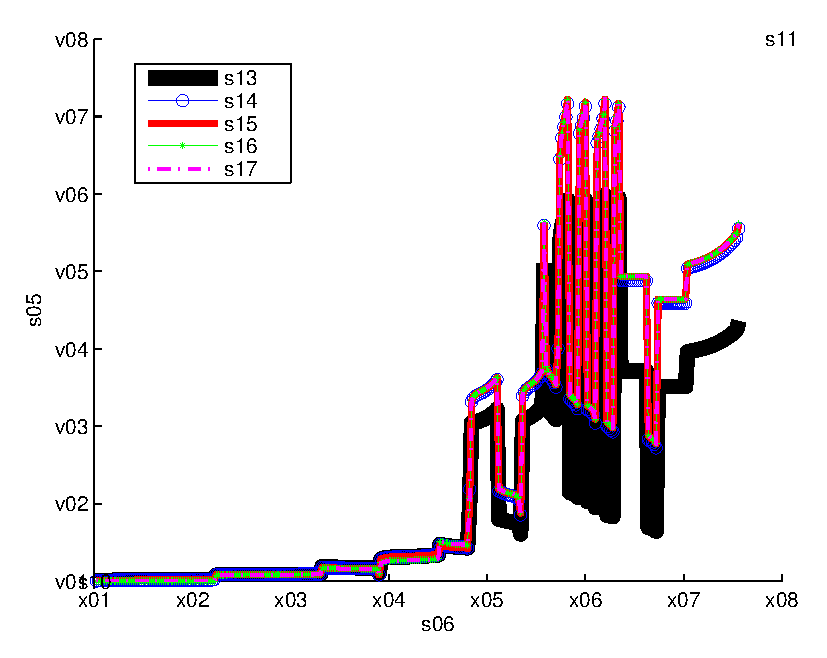
\includegraphics[width=15cm]{rmse_300_64.eps}%
\end{psfrags}%
%
% End rmse_300_64.tex
\end{document}
% See http://www.mathworks.de/matlabcentral/fileexchange/loadFile.do?objectId=4638
% for recent versions of laprint.m.
%
% created by:           LaPrint version 3.16 (13.9.2004)
% created on:           22-Apr-2014 13:54:10
% eps bounding box:     15 cm x 19.9821 cm
% comment:              
%
\begin{psfrags}%
\psfragscanon%
%
% text strings:
\psfrag{s14}[b][b]{\color[rgb]{0,0,0}\setlength{\tabcolsep}{0pt}\begin{tabular}{c}EKF\end{tabular}}%
\psfrag{s15}[b][b]{\color[rgb]{0,0,0}\setlength{\tabcolsep}{0pt}\begin{tabular}{c}UKF\end{tabular}}%
\psfrag{s16}[b][b]{\color[rgb]{0,0,0}\setlength{\tabcolsep}{0pt}\begin{tabular}{c}RMSE\end{tabular}}%
\psfrag{s17}[b][b]{\color[rgb]{0,0,0}\setlength{\tabcolsep}{0pt}\begin{tabular}{c}CKF3\end{tabular}}%
\psfrag{s18}[b][b]{\color[rgb]{0,0,0}\setlength{\tabcolsep}{0pt}\begin{tabular}{c}CKF5\end{tabular}}%
\psfrag{s19}[b][b]{\color[rgb]{0,0,0}\setlength{\tabcolsep}{0pt}\begin{tabular}{c}SLF\end{tabular}}%
\psfrag{s20}[t][t]{\color[rgb]{0,0,0}\setlength{\tabcolsep}{0pt}\begin{tabular}{c}$k$\end{tabular}}%
%
% xticklabels:
\psfrag{x01}[t][t]{0}%
\psfrag{x02}[t][t]{50}%
\psfrag{x03}[t][t]{100}%
\psfrag{x04}[t][t]{150}%
\psfrag{x05}[t][t]{200}%
\psfrag{x06}[t][t]{250}%
\psfrag{x07}[t][t]{300}%
\psfrag{x08}[t][t]{350}%
\psfrag{x09}[t][t]{0}%
\psfrag{x10}[t][t]{50}%
\psfrag{x11}[t][t]{100}%
\psfrag{x12}[t][t]{150}%
\psfrag{x13}[t][t]{200}%
\psfrag{x14}[t][t]{250}%
\psfrag{x15}[t][t]{300}%
\psfrag{x16}[t][t]{350}%
\psfrag{x17}[t][t]{0}%
\psfrag{x18}[t][t]{50}%
\psfrag{x19}[t][t]{100}%
\psfrag{x20}[t][t]{150}%
\psfrag{x21}[t][t]{200}%
\psfrag{x22}[t][t]{250}%
\psfrag{x23}[t][t]{300}%
\psfrag{x24}[t][t]{350}%
\psfrag{x25}[t][t]{0}%
\psfrag{x26}[t][t]{50}%
\psfrag{x27}[t][t]{100}%
\psfrag{x28}[t][t]{150}%
\psfrag{x29}[t][t]{200}%
\psfrag{x30}[t][t]{250}%
\psfrag{x31}[t][t]{300}%
\psfrag{x32}[t][t]{350}%
\psfrag{x33}[t][t]{0}%
\psfrag{x34}[t][t]{50}%
\psfrag{x35}[t][t]{100}%
\psfrag{x36}[t][t]{150}%
\psfrag{x37}[t][t]{200}%
\psfrag{x38}[t][t]{250}%
\psfrag{x39}[t][t]{300}%
\psfrag{x40}[t][t]{350}%
%
% yticklabels:
\psfrag{v01}[r][r]{0}%
\psfrag{v02}[r][r]{0.02}%
\psfrag{v03}[r][r]{0.04}%
\psfrag{v04}[r][r]{0}%
\psfrag{v05}[r][r]{0.02}%
\psfrag{v06}[r][r]{0.04}%
\psfrag{v07}[r][r]{0}%
\psfrag{v08}[r][r]{0.02}%
\psfrag{v09}[r][r]{0.04}%
\psfrag{v10}[r][r]{0}%
\psfrag{v11}[r][r]{0.02}%
\psfrag{v12}[r][r]{0.04}%
\psfrag{v13}[r][r]{0}%
\psfrag{v14}[r][r]{0.02}%
\psfrag{v15}[r][r]{0.04}%
%
% Figure:
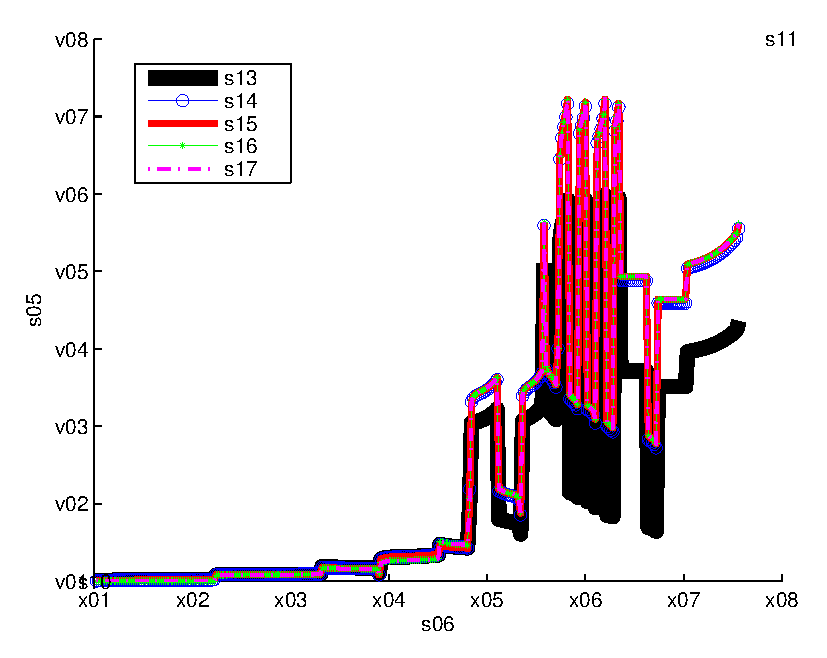
\includegraphics[width=15cm]{rmse_300_64.eps}%
\end{psfrags}%
%
% End rmse_300_64.tex
\end{document}
% See http://www.mathworks.de/matlabcentral/fileexchange/loadFile.do?objectId=4638
% for recent versions of laprint.m.
%
% created by:           LaPrint version 3.16 (13.9.2004)
% created on:           22-Apr-2014 13:54:10
% eps bounding box:     15 cm x 19.9821 cm
% comment:              
%
\begin{psfrags}%
\psfragscanon%
%
% text strings:
\psfrag{s14}[b][b]{\color[rgb]{0,0,0}\setlength{\tabcolsep}{0pt}\begin{tabular}{c}EKF\end{tabular}}%
\psfrag{s15}[b][b]{\color[rgb]{0,0,0}\setlength{\tabcolsep}{0pt}\begin{tabular}{c}UKF\end{tabular}}%
\psfrag{s16}[b][b]{\color[rgb]{0,0,0}\setlength{\tabcolsep}{0pt}\begin{tabular}{c}RMSE\end{tabular}}%
\psfrag{s17}[b][b]{\color[rgb]{0,0,0}\setlength{\tabcolsep}{0pt}\begin{tabular}{c}CKF3\end{tabular}}%
\psfrag{s18}[b][b]{\color[rgb]{0,0,0}\setlength{\tabcolsep}{0pt}\begin{tabular}{c}CKF5\end{tabular}}%
\psfrag{s19}[b][b]{\color[rgb]{0,0,0}\setlength{\tabcolsep}{0pt}\begin{tabular}{c}SLF\end{tabular}}%
\psfrag{s20}[t][t]{\color[rgb]{0,0,0}\setlength{\tabcolsep}{0pt}\begin{tabular}{c}$k$\end{tabular}}%
%
% xticklabels:
\psfrag{x01}[t][t]{0}%
\psfrag{x02}[t][t]{50}%
\psfrag{x03}[t][t]{100}%
\psfrag{x04}[t][t]{150}%
\psfrag{x05}[t][t]{200}%
\psfrag{x06}[t][t]{250}%
\psfrag{x07}[t][t]{300}%
\psfrag{x08}[t][t]{350}%
\psfrag{x09}[t][t]{0}%
\psfrag{x10}[t][t]{50}%
\psfrag{x11}[t][t]{100}%
\psfrag{x12}[t][t]{150}%
\psfrag{x13}[t][t]{200}%
\psfrag{x14}[t][t]{250}%
\psfrag{x15}[t][t]{300}%
\psfrag{x16}[t][t]{350}%
\psfrag{x17}[t][t]{0}%
\psfrag{x18}[t][t]{50}%
\psfrag{x19}[t][t]{100}%
\psfrag{x20}[t][t]{150}%
\psfrag{x21}[t][t]{200}%
\psfrag{x22}[t][t]{250}%
\psfrag{x23}[t][t]{300}%
\psfrag{x24}[t][t]{350}%
\psfrag{x25}[t][t]{0}%
\psfrag{x26}[t][t]{50}%
\psfrag{x27}[t][t]{100}%
\psfrag{x28}[t][t]{150}%
\psfrag{x29}[t][t]{200}%
\psfrag{x30}[t][t]{250}%
\psfrag{x31}[t][t]{300}%
\psfrag{x32}[t][t]{350}%
\psfrag{x33}[t][t]{0}%
\psfrag{x34}[t][t]{50}%
\psfrag{x35}[t][t]{100}%
\psfrag{x36}[t][t]{150}%
\psfrag{x37}[t][t]{200}%
\psfrag{x38}[t][t]{250}%
\psfrag{x39}[t][t]{300}%
\psfrag{x40}[t][t]{350}%
%
% yticklabels:
\psfrag{v01}[r][r]{0}%
\psfrag{v02}[r][r]{0.02}%
\psfrag{v03}[r][r]{0.04}%
\psfrag{v04}[r][r]{0}%
\psfrag{v05}[r][r]{0.02}%
\psfrag{v06}[r][r]{0.04}%
\psfrag{v07}[r][r]{0}%
\psfrag{v08}[r][r]{0.02}%
\psfrag{v09}[r][r]{0.04}%
\psfrag{v10}[r][r]{0}%
\psfrag{v11}[r][r]{0.02}%
\psfrag{v12}[r][r]{0.04}%
\psfrag{v13}[r][r]{0}%
\psfrag{v14}[r][r]{0.02}%
\psfrag{v15}[r][r]{0.04}%
%
% Figure:
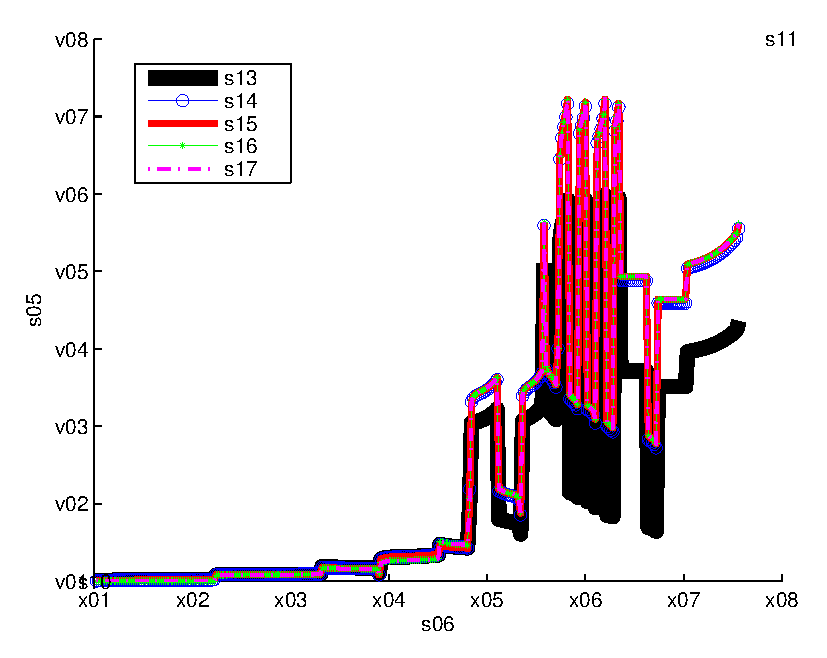
\includegraphics[width=15cm]{rmse_300_64.eps}%
\end{psfrags}%
%
% End rmse_300_64.tex

\pstool[width=15cm]{chapter-3/figures/rmse_300_64}{% This file is generated by the MATLAB m-file laprint.m. It can be included
% into LaTeX documents using the packages graphicx, color and psfrag.
% It is accompanied by a postscript file. A sample LaTeX file is:
%    \documentclass{article}\usepackage{graphicx,color,psfrag}
%    \begin{document}% This file is generated by the MATLAB m-file laprint.m. It can be included
% into LaTeX documents using the packages graphicx, color and psfrag.
% It is accompanied by a postscript file. A sample LaTeX file is:
%    \documentclass{article}\usepackage{graphicx,color,psfrag}
%    \begin{document}% This file is generated by the MATLAB m-file laprint.m. It can be included
% into LaTeX documents using the packages graphicx, color and psfrag.
% It is accompanied by a postscript file. A sample LaTeX file is:
%    \documentclass{article}\usepackage{graphicx,color,psfrag}
%    \begin{document}\input{rmse_300_64}\end{document}
% See http://www.mathworks.de/matlabcentral/fileexchange/loadFile.do?objectId=4638
% for recent versions of laprint.m.
%
% created by:           LaPrint version 3.16 (13.9.2004)
% created on:           22-Apr-2014 13:54:10
% eps bounding box:     15 cm x 19.9821 cm
% comment:              
%
\begin{psfrags}%
\psfragscanon%
%
% text strings:
\psfrag{s14}[b][b]{\color[rgb]{0,0,0}\setlength{\tabcolsep}{0pt}\begin{tabular}{c}EKF\end{tabular}}%
\psfrag{s15}[b][b]{\color[rgb]{0,0,0}\setlength{\tabcolsep}{0pt}\begin{tabular}{c}UKF\end{tabular}}%
\psfrag{s16}[b][b]{\color[rgb]{0,0,0}\setlength{\tabcolsep}{0pt}\begin{tabular}{c}RMSE\end{tabular}}%
\psfrag{s17}[b][b]{\color[rgb]{0,0,0}\setlength{\tabcolsep}{0pt}\begin{tabular}{c}CKF3\end{tabular}}%
\psfrag{s18}[b][b]{\color[rgb]{0,0,0}\setlength{\tabcolsep}{0pt}\begin{tabular}{c}CKF5\end{tabular}}%
\psfrag{s19}[b][b]{\color[rgb]{0,0,0}\setlength{\tabcolsep}{0pt}\begin{tabular}{c}SLF\end{tabular}}%
\psfrag{s20}[t][t]{\color[rgb]{0,0,0}\setlength{\tabcolsep}{0pt}\begin{tabular}{c}$k$\end{tabular}}%
%
% xticklabels:
\psfrag{x01}[t][t]{0}%
\psfrag{x02}[t][t]{50}%
\psfrag{x03}[t][t]{100}%
\psfrag{x04}[t][t]{150}%
\psfrag{x05}[t][t]{200}%
\psfrag{x06}[t][t]{250}%
\psfrag{x07}[t][t]{300}%
\psfrag{x08}[t][t]{350}%
\psfrag{x09}[t][t]{0}%
\psfrag{x10}[t][t]{50}%
\psfrag{x11}[t][t]{100}%
\psfrag{x12}[t][t]{150}%
\psfrag{x13}[t][t]{200}%
\psfrag{x14}[t][t]{250}%
\psfrag{x15}[t][t]{300}%
\psfrag{x16}[t][t]{350}%
\psfrag{x17}[t][t]{0}%
\psfrag{x18}[t][t]{50}%
\psfrag{x19}[t][t]{100}%
\psfrag{x20}[t][t]{150}%
\psfrag{x21}[t][t]{200}%
\psfrag{x22}[t][t]{250}%
\psfrag{x23}[t][t]{300}%
\psfrag{x24}[t][t]{350}%
\psfrag{x25}[t][t]{0}%
\psfrag{x26}[t][t]{50}%
\psfrag{x27}[t][t]{100}%
\psfrag{x28}[t][t]{150}%
\psfrag{x29}[t][t]{200}%
\psfrag{x30}[t][t]{250}%
\psfrag{x31}[t][t]{300}%
\psfrag{x32}[t][t]{350}%
\psfrag{x33}[t][t]{0}%
\psfrag{x34}[t][t]{50}%
\psfrag{x35}[t][t]{100}%
\psfrag{x36}[t][t]{150}%
\psfrag{x37}[t][t]{200}%
\psfrag{x38}[t][t]{250}%
\psfrag{x39}[t][t]{300}%
\psfrag{x40}[t][t]{350}%
%
% yticklabels:
\psfrag{v01}[r][r]{0}%
\psfrag{v02}[r][r]{0.02}%
\psfrag{v03}[r][r]{0.04}%
\psfrag{v04}[r][r]{0}%
\psfrag{v05}[r][r]{0.02}%
\psfrag{v06}[r][r]{0.04}%
\psfrag{v07}[r][r]{0}%
\psfrag{v08}[r][r]{0.02}%
\psfrag{v09}[r][r]{0.04}%
\psfrag{v10}[r][r]{0}%
\psfrag{v11}[r][r]{0.02}%
\psfrag{v12}[r][r]{0.04}%
\psfrag{v13}[r][r]{0}%
\psfrag{v14}[r][r]{0.02}%
\psfrag{v15}[r][r]{0.04}%
%
% Figure:
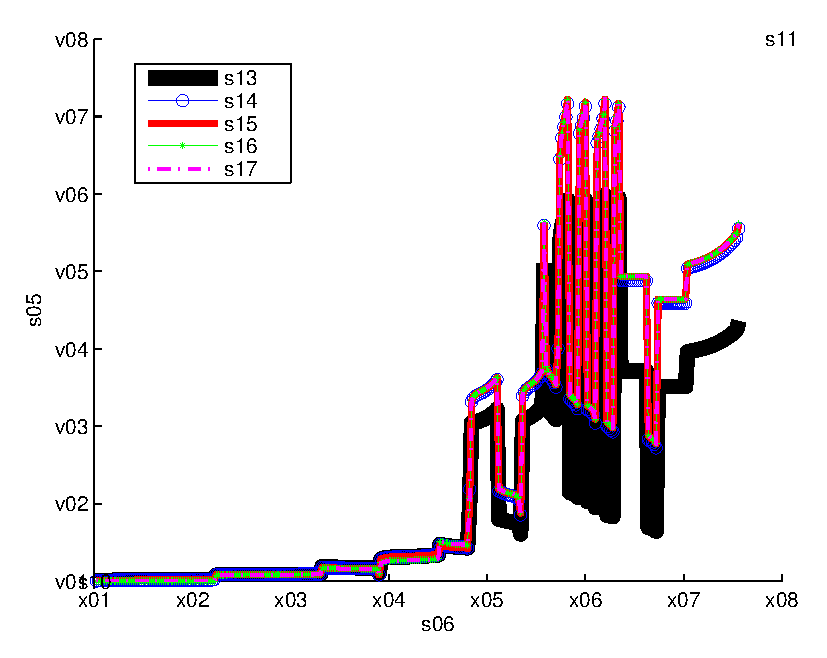
\includegraphics[width=15cm]{rmse_300_64.eps}%
\end{psfrags}%
%
% End rmse_300_64.tex
\end{document}
% See http://www.mathworks.de/matlabcentral/fileexchange/loadFile.do?objectId=4638
% for recent versions of laprint.m.
%
% created by:           LaPrint version 3.16 (13.9.2004)
% created on:           22-Apr-2014 13:54:10
% eps bounding box:     15 cm x 19.9821 cm
% comment:              
%
\begin{psfrags}%
\psfragscanon%
%
% text strings:
\psfrag{s14}[b][b]{\color[rgb]{0,0,0}\setlength{\tabcolsep}{0pt}\begin{tabular}{c}EKF\end{tabular}}%
\psfrag{s15}[b][b]{\color[rgb]{0,0,0}\setlength{\tabcolsep}{0pt}\begin{tabular}{c}UKF\end{tabular}}%
\psfrag{s16}[b][b]{\color[rgb]{0,0,0}\setlength{\tabcolsep}{0pt}\begin{tabular}{c}RMSE\end{tabular}}%
\psfrag{s17}[b][b]{\color[rgb]{0,0,0}\setlength{\tabcolsep}{0pt}\begin{tabular}{c}CKF3\end{tabular}}%
\psfrag{s18}[b][b]{\color[rgb]{0,0,0}\setlength{\tabcolsep}{0pt}\begin{tabular}{c}CKF5\end{tabular}}%
\psfrag{s19}[b][b]{\color[rgb]{0,0,0}\setlength{\tabcolsep}{0pt}\begin{tabular}{c}SLF\end{tabular}}%
\psfrag{s20}[t][t]{\color[rgb]{0,0,0}\setlength{\tabcolsep}{0pt}\begin{tabular}{c}$k$\end{tabular}}%
%
% xticklabels:
\psfrag{x01}[t][t]{0}%
\psfrag{x02}[t][t]{50}%
\psfrag{x03}[t][t]{100}%
\psfrag{x04}[t][t]{150}%
\psfrag{x05}[t][t]{200}%
\psfrag{x06}[t][t]{250}%
\psfrag{x07}[t][t]{300}%
\psfrag{x08}[t][t]{350}%
\psfrag{x09}[t][t]{0}%
\psfrag{x10}[t][t]{50}%
\psfrag{x11}[t][t]{100}%
\psfrag{x12}[t][t]{150}%
\psfrag{x13}[t][t]{200}%
\psfrag{x14}[t][t]{250}%
\psfrag{x15}[t][t]{300}%
\psfrag{x16}[t][t]{350}%
\psfrag{x17}[t][t]{0}%
\psfrag{x18}[t][t]{50}%
\psfrag{x19}[t][t]{100}%
\psfrag{x20}[t][t]{150}%
\psfrag{x21}[t][t]{200}%
\psfrag{x22}[t][t]{250}%
\psfrag{x23}[t][t]{300}%
\psfrag{x24}[t][t]{350}%
\psfrag{x25}[t][t]{0}%
\psfrag{x26}[t][t]{50}%
\psfrag{x27}[t][t]{100}%
\psfrag{x28}[t][t]{150}%
\psfrag{x29}[t][t]{200}%
\psfrag{x30}[t][t]{250}%
\psfrag{x31}[t][t]{300}%
\psfrag{x32}[t][t]{350}%
\psfrag{x33}[t][t]{0}%
\psfrag{x34}[t][t]{50}%
\psfrag{x35}[t][t]{100}%
\psfrag{x36}[t][t]{150}%
\psfrag{x37}[t][t]{200}%
\psfrag{x38}[t][t]{250}%
\psfrag{x39}[t][t]{300}%
\psfrag{x40}[t][t]{350}%
%
% yticklabels:
\psfrag{v01}[r][r]{0}%
\psfrag{v02}[r][r]{0.02}%
\psfrag{v03}[r][r]{0.04}%
\psfrag{v04}[r][r]{0}%
\psfrag{v05}[r][r]{0.02}%
\psfrag{v06}[r][r]{0.04}%
\psfrag{v07}[r][r]{0}%
\psfrag{v08}[r][r]{0.02}%
\psfrag{v09}[r][r]{0.04}%
\psfrag{v10}[r][r]{0}%
\psfrag{v11}[r][r]{0.02}%
\psfrag{v12}[r][r]{0.04}%
\psfrag{v13}[r][r]{0}%
\psfrag{v14}[r][r]{0.02}%
\psfrag{v15}[r][r]{0.04}%
%
% Figure:
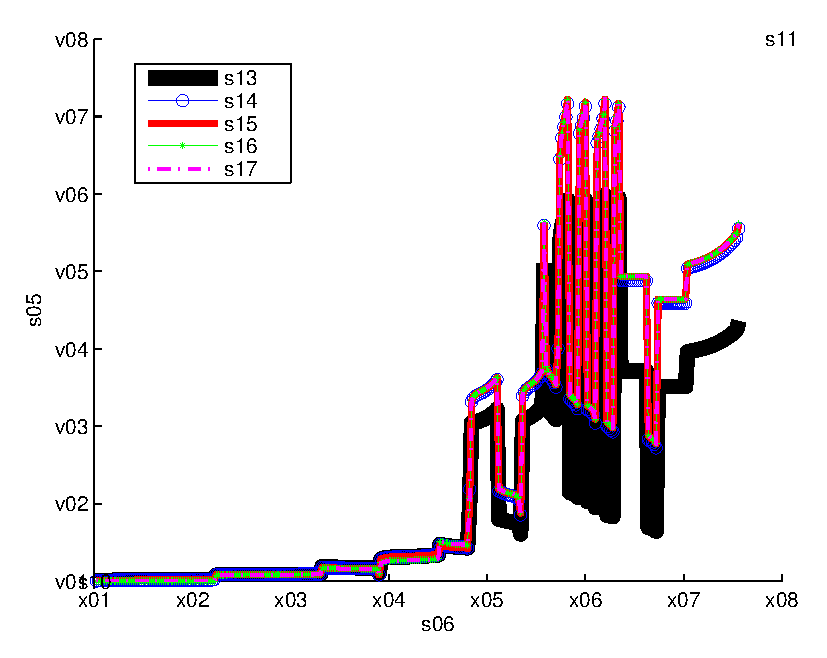
\includegraphics[width=15cm]{rmse_300_64.eps}%
\end{psfrags}%
%
% End rmse_300_64.tex
\end{document}
% See http://www.mathworks.de/matlabcentral/fileexchange/loadFile.do?objectId=4638
% for recent versions of laprint.m.
%
% created by:           LaPrint version 3.16 (13.9.2004)
% created on:           22-Apr-2014 13:54:10
% eps bounding box:     15 cm x 19.9821 cm
% comment:              
%
\begin{psfrags}%
\psfragscanon%
%
% text strings:
\psfrag{s14}[b][b]{\color[rgb]{0,0,0}\setlength{\tabcolsep}{0pt}\begin{tabular}{c}EKF\end{tabular}}%
\psfrag{s15}[b][b]{\color[rgb]{0,0,0}\setlength{\tabcolsep}{0pt}\begin{tabular}{c}UKF\end{tabular}}%
\psfrag{s16}[b][b]{\color[rgb]{0,0,0}\setlength{\tabcolsep}{0pt}\begin{tabular}{c}RMSE\end{tabular}}%
\psfrag{s17}[b][b]{\color[rgb]{0,0,0}\setlength{\tabcolsep}{0pt}\begin{tabular}{c}CKF3\end{tabular}}%
\psfrag{s18}[b][b]{\color[rgb]{0,0,0}\setlength{\tabcolsep}{0pt}\begin{tabular}{c}CKF5\end{tabular}}%
\psfrag{s19}[b][b]{\color[rgb]{0,0,0}\setlength{\tabcolsep}{0pt}\begin{tabular}{c}SLF\end{tabular}}%
\psfrag{s20}[t][t]{\color[rgb]{0,0,0}\setlength{\tabcolsep}{0pt}\begin{tabular}{c}$k$\end{tabular}}%
%
% xticklabels:
\psfrag{x01}[t][t]{0}%
\psfrag{x02}[t][t]{50}%
\psfrag{x03}[t][t]{100}%
\psfrag{x04}[t][t]{150}%
\psfrag{x05}[t][t]{200}%
\psfrag{x06}[t][t]{250}%
\psfrag{x07}[t][t]{300}%
\psfrag{x08}[t][t]{350}%
\psfrag{x09}[t][t]{0}%
\psfrag{x10}[t][t]{50}%
\psfrag{x11}[t][t]{100}%
\psfrag{x12}[t][t]{150}%
\psfrag{x13}[t][t]{200}%
\psfrag{x14}[t][t]{250}%
\psfrag{x15}[t][t]{300}%
\psfrag{x16}[t][t]{350}%
\psfrag{x17}[t][t]{0}%
\psfrag{x18}[t][t]{50}%
\psfrag{x19}[t][t]{100}%
\psfrag{x20}[t][t]{150}%
\psfrag{x21}[t][t]{200}%
\psfrag{x22}[t][t]{250}%
\psfrag{x23}[t][t]{300}%
\psfrag{x24}[t][t]{350}%
\psfrag{x25}[t][t]{0}%
\psfrag{x26}[t][t]{50}%
\psfrag{x27}[t][t]{100}%
\psfrag{x28}[t][t]{150}%
\psfrag{x29}[t][t]{200}%
\psfrag{x30}[t][t]{250}%
\psfrag{x31}[t][t]{300}%
\psfrag{x32}[t][t]{350}%
\psfrag{x33}[t][t]{0}%
\psfrag{x34}[t][t]{50}%
\psfrag{x35}[t][t]{100}%
\psfrag{x36}[t][t]{150}%
\psfrag{x37}[t][t]{200}%
\psfrag{x38}[t][t]{250}%
\psfrag{x39}[t][t]{300}%
\psfrag{x40}[t][t]{350}%
%
% yticklabels:
\psfrag{v01}[r][r]{0}%
\psfrag{v02}[r][r]{0.02}%
\psfrag{v03}[r][r]{0.04}%
\psfrag{v04}[r][r]{0}%
\psfrag{v05}[r][r]{0.02}%
\psfrag{v06}[r][r]{0.04}%
\psfrag{v07}[r][r]{0}%
\psfrag{v08}[r][r]{0.02}%
\psfrag{v09}[r][r]{0.04}%
\psfrag{v10}[r][r]{0}%
\psfrag{v11}[r][r]{0.02}%
\psfrag{v12}[r][r]{0.04}%
\psfrag{v13}[r][r]{0}%
\psfrag{v14}[r][r]{0.02}%
\psfrag{v15}[r][r]{0.04}%
%
% Figure:
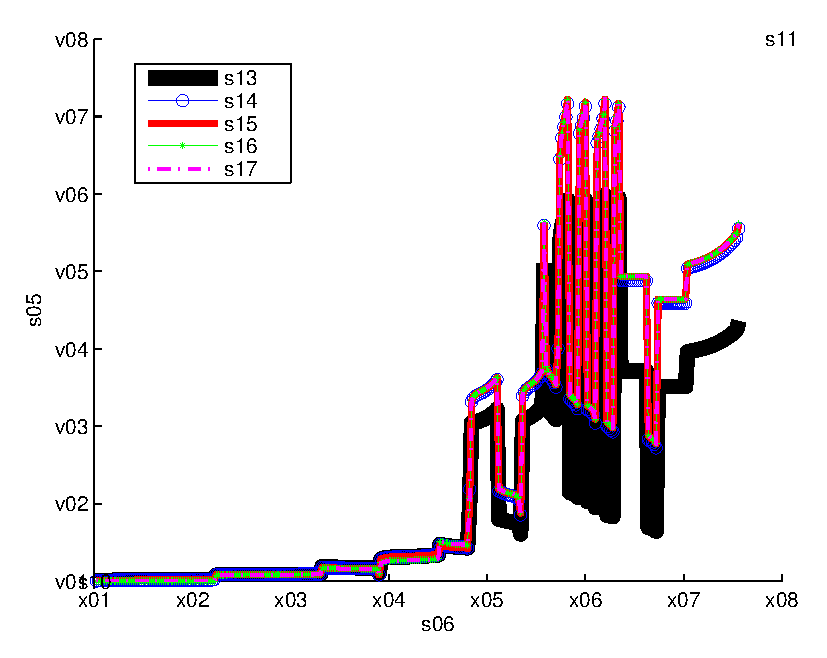
\includegraphics[width=15cm]{rmse_300_64.eps}%
\end{psfrags}%
%
% End rmse_300_64.tex
}
\caption{RMSE of SOC estimation for $T_s=300$~s and $M=64$.}
\label{fig:rmse_300_64}
\end{figure}

\begin{figure}
\centering
%\input{chapter-3/figures/rmse_300_256}
\pstool[width=15cm]{chapter-3/figures/rmse_300_256}{\input{chapter-3/figures/rmse_300_256.tex}}
\caption{RMSE of SOC estimation for $T_s=300$~s and $M=256$.}
\label{fig:rmse_300_256}
\end{figure}

\end{document}
